\chapter{Voting by Local Visual-temporal Patterns for Efficient Thermal Feature Detection in Tunnels}
\label{chp3}

\section{Introduction}

From time to time, efficient detection methods under limited computational power are important in various areas, such as driving assistance using embedded sensors. In this chapter, a method pursuing efficiency and real-time detection is proposed.
The proposed detection method makes use of both
appearance and motion information of the target objects. By well optimizing the detecting pipeline, the
method works in real time, and gives promising detection results in experiments  carried on data collected by infrared cameras.

As always, detection performance and efficiency are the two important aspects of this method.
In a tunnel environment, in addition to the target objects, a lot of noisy objects also appear, e.g. ordinary lights, other vehicles, and other vehicles' shadows. And some of the noisy objects cannot even be distinguished from the target objects by appearance , as shown in Figure \ref{fig:first}. The clutter property of the sensed data makes the detection challenging.
The proposed method meets this challenge by making use of both appearance and temporal information of the target objects.
There are three main steps in the method.

The first step deals with keypoints. It takes original data as input, and outputs keypoint clusters as detection hypotheses. In this step, keypoints are detected, verified and then clustered. To detect keypoints, all points on each frame are uniformly sampled and filtered with pre-set intensity thresholds.  Then the keypoints are verified by a simple keypoint appearance model   built by \emph{k}-means. At the end of the first step, the keypoints are clustered based on the Euclidean distance.

The second step takes the keypoint clusters as input, verifies them by appearance and temporal information, and outputs the keypoints which pass verification, as detection results. In the second step, the keypoint clusters are labeled based on appearance by an Adaboost machine, which is trained using intensity histograms of keypoint clusters from target objects and keypoint clusters from noisy objects. The keypoint clusters are also tracked by temporal association through frames. Motion information encoded in the trajectories are used to further verify the keypoint clusters. At the end of this step, the keypoint clustered are labeled as positive or negative according to whether they pass both appearance and motion verifications.

Voting systems are employed in the last step. The output of the second step are some keypoint clusters that pass both appearance and motion verifications. These keypoint clusters are connected by trajectories. Voting is carried on along each trajectory when it ends. If the percentage of positive keypoint clusters connected by one trajectory is larger than a threshold, this trajectory is then considered as an emergency telephone indicator.



This pipeline is also designed  with consideration for the requirement of efficiency.  The method deals with the large amounts of information contained on one frame, following a hierarchical manner. The later a step is, the more time-consuming it is, and the fewer instances it deals with. From an image containing $10^5$ pixels, $10^4$ points go through the keypoint detection step of testing by intensity thresholds. Then in average, $10^3$ keypoints are detected, and verified, leaving about $10^2$ keypoints to be clustered. Afterwards, fewer than $10$ keypoint clusters are left; these are dealt with by the very time-consuming steps of generating image features and tracking.

The advantage of this method is its ability to give promising detection results from cluttered data in real time. In addition, this method successfully  combines bottom-up and classification methods, as well as combines both appearance and temporal information.





This chapter is organized as follows. Section \ref{rw} reviews related work. Section \ref{ab} introduces application background. Section \ref{pip} proposes a pipeline for the method. Section \ref{exp} gives experimental results. Section \ref{ord} gives results by extending the method for data collected by ordinary cameras. Section \ref{conc} concludes.














\begin{figure}
\centering
\subfigure[]{
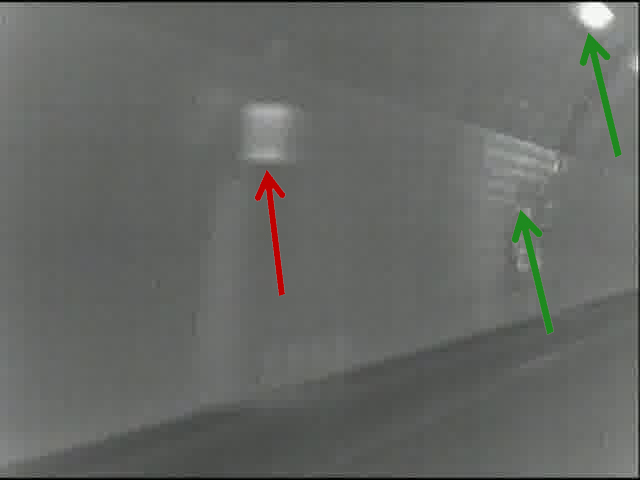
\includegraphics[width=0.47\textwidth,bb=0 0 640 480]{17Orgimg00039.jpg}
\label{fig:first:a}}
\subfigure[]{
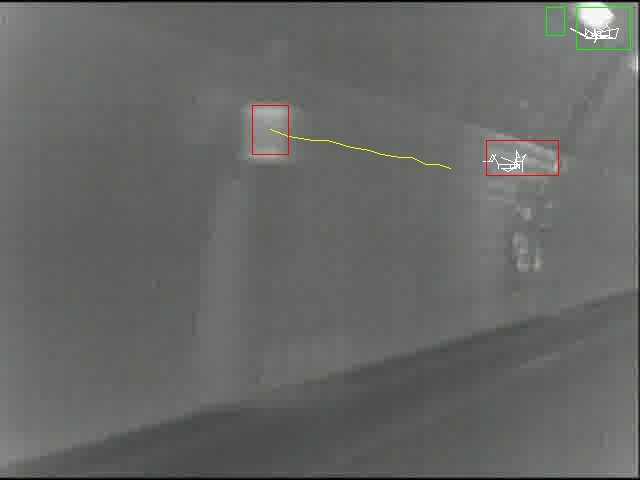
\includegraphics[width=0.47\textwidth,bb=0 0 640 480]{17veriTrjimg00039.jpg}
\label{fig:first:b}}
\caption[Target objects and detection results]{Original data and detection results. In (a), the red arrow points to the target object: emergency telephone indicator, and the green arrows point to noisy objects. In (b), red rectangles mark detection hypotheses labeled as positive using appearance information, and green rectangles mark negative ones. Yellow trajectories mark detection hypotheses labeled as positive using temporal information, and white trajectories mark negative ones.
}
\label{fig:first}
\end{figure}









\section{Related Work}
\label{rw}


Most modern detection methods fall into two categories. Some~\citep{ij4,ac31,ac30,ac4,ac32,ac29,ac28,ac1} follow the sliding-window schema, and they detect objects by considering whether each of the sub-images contains an instance of the target object. Classifiers are usually employed by these methods. The other methods~\citep{ac9,ac2,ac3,ac5,ac10,ac21,ac18} infer object centers based on local image features in a bottom-up manner. The proposed method takes advantages of both frameworks. Following the bottom-up manner, keypoints are detected, verified, and clustered. After these steps, the keypoint clusters are considered as detection hypotheses. Then following the sliding-window schema, the keypoint clusters are verified by their appearance and temporal information, using discriminative methods.

Previous methods~\citep{ac34} also consider the combination of the two frameworks. Detection hypotheses are gained using a Hough transform method and then verified by support vector machines in~\citep{ac10,ac25}. The methods in~\citep{ac6,ac7}, use randomized decision trees for both decisions: whether local features belong to foreground objects, and decisions of their Hough votes. The method proposed in~\citep{ac27} describes both frameworks in the same manner. While giving state-of-the-art detection performance, these other methods can't meet the requirement for efficiency as this method does.







This work is also related to data association methods at time dimension. In tracking, the main attention is focused on solving a data
association problem to explain conflicts in data as well as
recovering from tracking failures within a low time cost. In
\citep{ij9}, the joint likelihood maximization is represented by the
Nash Equilibrium in a game. The main contribution is that the time
complexity of solving a game-theoretic problem is low and this makes it efficient to
solve conflicts between trackers. In
\citep{ij10}, the problem of maximum a posteriori is embedded to the max flow of a well designed
graph. And it is able to recover
missed detections on middle frames and works efficiently. In
\citep{my7}, the main idea is to firstly connect very faithful
detection response pairs, then solve the data association problem
via low-time-complexity Hungarian algorithm, and refine the results
in an expectation-maximization manner in later steps. And the most important concern of these methods
is finding efficient solutions in   data association problems.

This work is also related to feature grouping methods~\citep{ac25}, detecting methods using trajectories~\citep{my9,ac24}, tracking methods~\citep{my7,my10}, and methods integrating appearance and temporal information~\citep{ac23}.




\section{Application background}
\label{ab}

When developing the method, potential application scenarios are within consideration. The method aims to perform detection in real time, and serve as an effective unit in positioning automobiles in tunnel environment.


Positioning of vehicles acts as a fundamental role in autonomous driving, and is also of great importance for driving assistance, vehicle navigation, etc. When GPS sensors function properly, the task is easy. While in a tunnel environment, there are no GPS signals available for most of the time. A new positioning system which functions properly in a tunnel environment is necessary~\citep{nig}. An object detection method which can be used for positioning systems in tunnels is here proposed.

This method is part of an automated driving system in a NEDO project, "Development of Energy-saving ITS Technologies".
The automated driving system is vehicle-oriented, and an express way is the main application scenario. No specific facilities are assumed to exist on road sides, while instead, the experimental vehicles are equipped with  sensors and vehicle-to-vehicle communication systems. There are a few sensors used for positioning. For example, sensors used to extract white road lines to estimate the lateral position in the lane, GPS sensors, dead reckoning systems, and stereo far-infrared camera systems intended for obstacle detection. On the street, GPS sensors can be used for positioning. While positioning in tunnels is difficult since GPS signals are not available and no specific equipment on road sides is assumed. For positioning in tunnels, GPS sensors are used to record the position of  tunnel entrances, and dead reckoning systems are used to infer position by continuously sensing the vehicles' speed and direction. However, errors of dead reckoning systems will accumulate. Thus, the proposed method uses far-infrared cameras installed on the vehicles to detect signs in the tunnels, which contain position information, and will be used to eliminate the accumulated errors.

In most tunnels   on the expressways in Japan, there are many signs appearing at equal intervals. The method focuses on the emergency telephone indicators, which appear every 200 meters in tunnels. The absolute coordinates of the emergency telephone indicators can be obtained by the method of~\citep{xue}.  If the emergency telephone indicators can be sensed while traveling in tunnels, and the distance from the vehicle to the indicators can be estimated,  then this information  can be used to eliminate accumulated errors of dead reckoning systems.
Detection methods, e.g.~\citep{ac23}, based on ordinary cameras fail due to darkness. Here the method uses far-infrared cameras,  which are suitable in dark environments and are already installed on our experimental vehicles.

 In a tunnel environment, besides the target objects, a lot of noisy objects also appear, e.g. ordinary lights, other vehicles, and other vehicles' shadows. So to well distinguish target objects is of importance. And such kind of applications usually require real-time detections. And the proposed method successfully meet the requirements.

\begin{comment}
Especially, compared with the method proposed in~\citep{wang1}, this method employs a more effective classifying machine by setting biased weights for positive and negative training examples, and far over-perform the method.
Inspired by a previous work~\citep{wang1}, the proposed method can be turned to an  approach to detecting emergency telephone indicators by using infrared cameras.
\end{comment}
\section{Detection Pipeline}
\label{pip}
The method can be considered as a three-step method. The first step deals with keypoints. It
takes original data as input, and outputs keypoint clusters as detection hypotheses. The second
step takes these keypoint clusters as input, verifies them by their appearance and motion
information, and labels them as positive or negative. In the third step, keypoint clusters connected by the same trajectory will vote for whether the trajectory is positive or negative when the trajectory ends, and this gives the final detection results of emergence telephone indicators.

\subsection{Keypoint Detection}

In data collected using ordinary cameras, keypoints~\citep{o2,o12} invariant to rotations, affine changes, and illumination changes are preferable. In this case, keypoint detection is intended to provide hypotheses for emergency telephone indicators. Thus intensity is of great importance. This method employs a simple yet useful method to detect keypoints. Firstly, points are uniformly sampled for an offset of 6 in width, and 7 in height (the length of an emergency telephone indicator is larger than its width). In this manner the magnitude of instances is reduced by nearly two orders. Then points that pass the test, which verifies them by setting intensity thresholds, are considered as keypoints.

Here a Gaussian distribution is assumed for the intensities of the points.




Let$\{\bf{x}\}$ denote all the sampled points, $I_{\bf{x}}$ the intensity of each point, \begin{comment}$I_{\bf{x}}\sim{\mathcal{N}(\mu_{I_{\bf{x}}},{\sigma_{I_{\bf{x}}}}^2)}$,
\end{comment}
and $l_{\bf{x}}$ the label. If the point is considered as belonging to target objects, $l_{\bf{x}}=1$, otherwise, $l_{\bf{x}}=0$. By setting lower threshold, $I^{th1}_{\bf{x}}$,  and higher threshold, $I^{th2}_{\bf{x}}$, the probability that points belongs to target objects based on their falling into this interval is given by,
\begin{equation}
P(l_{\bf{x}}=1|I^{th1}_{\bf{x}}{\leq}I_x{\leq}{I^{th2}_{\bf{x}}})=
\frac
{P(l_{\bf{x}}=1,I^{th1}_{\bf{x}}{\leq}I_x{\leq}{I^{th2}_{\bf{x}}})} {P(I^{th1}_{\bf{x}}{\leq}I_x{\leq}{I^{th2}_{\bf{x}}})}\;.
\label{eq1}
\end{equation}



At this step, the possibility that as few points as possible, belonging to the emergency telephone indicators, are excluded, is also considered. The probability of one point falling into the defined interval based on its belonging to emergency telephone indicators is given by,
\begin{equation}
P(I^{th1}_{\bf{x}}{\leq}I_x{\leq}{I^{th2}_{\bf{x}}}|l_{\bf{x}}=1)=
\frac
{P(l_{\bf{x}}=1,I^{th1}_{\bf{x}}{\leq}I_x{\leq}{I^{th2}_{\bf{x}}})} {P(l_{\bf{x}}=1)}\;.
\label{eq1.1}
\end{equation}
%del2
Points for which the intensities fall in the pre-set thresholds, are detected as keypoints.
\begin{figure}
\centering
\subfigure[]{
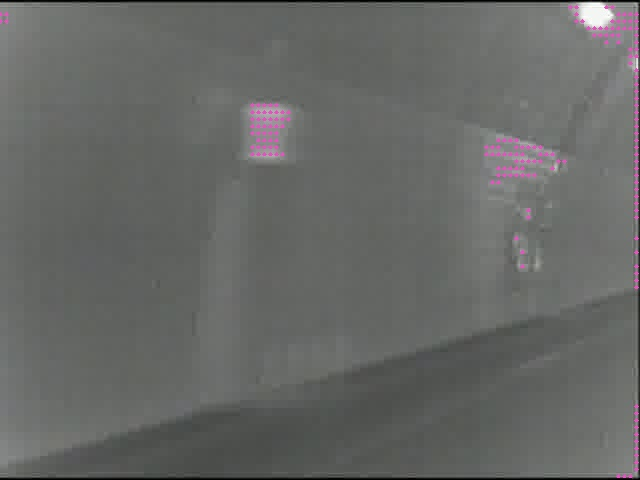
\includegraphics[width=0.47\textwidth,bb=0 0 640 480]{17Kptimg00039.jpg}
\label{fig:secc:a}}
\subfigure[]{
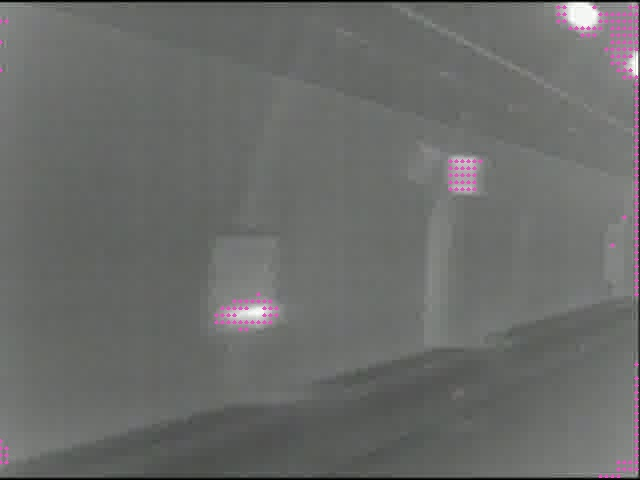
\includegraphics[width=0.47\textwidth,bb=0 0 640 480]{8Kptimg00028.jpg}
\label{fig:secc:b}}
\caption[Keypoint detection]{Keypoint detection. }
\label{fig:secc}
\end{figure}


\subsection{Keypoint Verification}


As shown in Figure \ref{fig:secc:b}, the detected keypoints don't just belong to emergency telephone indicators, but also belong to the background. For training purposes, keypoints belonging to emergency telephone indicators are considered  positive, all others are negative.

To verify the keypoints, the appearance of the sub-image around each keypoint is used. Intensity histograms are used to describe the appearance. Noisy keypoints not only come from the wall of the tunnel, but also from ordinary lights, other vehicles, and other vehicles' shadows. Thus robust linear classifiers are not suitable for the verification. Here, a general model in the form of a simple mixture is used. The \emph{k}-means method is used to cluster the intensity histograms, $\{A_{\bf{x}},l_{\bf{x}}=1\}$, of the positive keypoints, and, $\{A_{\bf{x}},l_{\bf{x}}=0\}$,  of
the negative keypoints.

Let $\{C_1^i,i=1,2,...,n_1\}$ denote the intensity histogram centers of the positive keypoints, and $\{C_0^i,i=1,2,...,n_2\}$ the negative. For each $C_1$, the average Euclidean distance between $\{C_0^i,i=1,2,...,n_2\}$ is calculated as,
\begin{equation}
Eu(C_1^i)={\frac 1 n_2}\sum\limits^{n_2}_{j=1}Euclid(C_1^i,C_0^j)\;.
\label{eq2}
\end{equation}
Here, $Euclid(\cdot)$ calculates the Euclidean distance, and $Eu(\cdot)$ is an evaluation function of the positive feature centers. The positive feature centers are ranked by $Eu(\cdot)$, and the 10 positive feature centers with the largest $Eu(\cdot)$ are chosen and used for verification.

For verification, the intensity histogram of each keypoint's surrounding sub-image is extracted. Then the Euclidean distance between the extracted intensity histogram and its nearest positive feature center is calculated. If this distance exceeds a threshold, $D^{th}_{A_{\bf{x}}}$, it is considered negative, otherwise it is considered positive. Here, for simplicity, unlike~\citep{ac33}, the same threshold is used for all components of the mixture.


\begin{figure}
\centering
\subfigure[]{
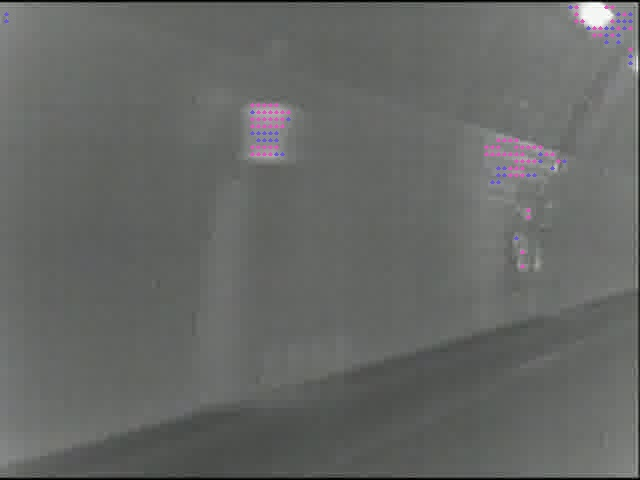
\includegraphics[width=0.47\textwidth,bb=0 0 640 480]{17VeriKptimg00039.jpg}
\label{fig:thirr:a}}
\subfigure[]{
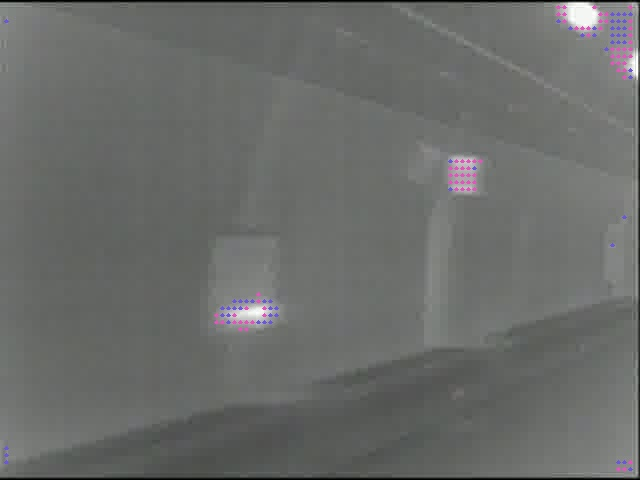
\includegraphics[width=0.47\textwidth,bb=0 0 640 480]{8VeriKptimg00028.jpg}
\label{fig:thirr:b}}
\subfigure[]{
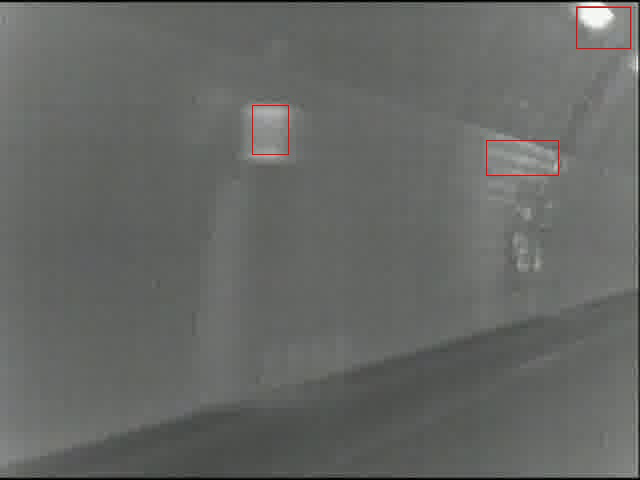
\includegraphics[width=0.47\textwidth,bb=0 0 640 480]{17Rgsimgwl00039.jpg}
\label{fig:thirr:c}}
\subfigure[]{
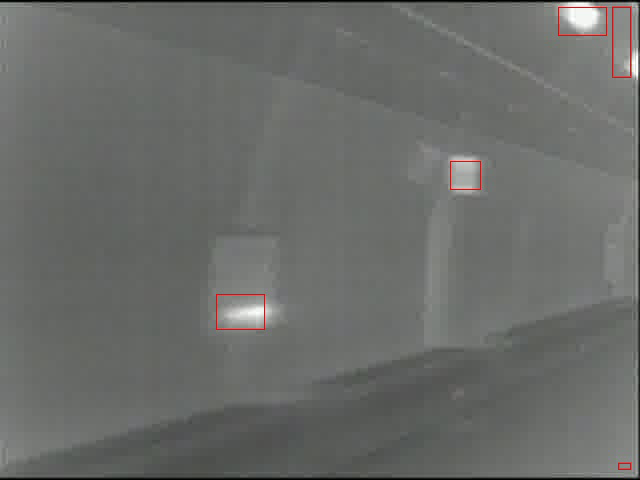
\includegraphics[width=0.47\textwidth,bb=0 0 640 480]{8Rgsimgwl00028.jpg}
\label{fig:thirr:d}}
\caption[Keypoint verification and clustering]{Keypoint verification and clustering. Red circles mark keypoints which pass the verification, while blue marks failed ones. Rectangles mark keypoint clustering results. }
\label{fig:thirr}
\end{figure}

\subsection{Keypoint Clustering}

After the keypoint verification step, on some frames the result is pretty good, while on other frames appearance of the keypoints is not enough to decide whether the keypoints belong to the emergency telephone indicators. Here generation of keypoint trajectories is not feasible, since nearby keypoints are similar in appearance and  the time complexity of associating such a large number of keypoints along the time dimension is high. So the keypoints are clustered, then data association in time dimension only is needed to deal with a small number of keypoint clusters.

To cluster the keypoints, a minimum spanning tree (mst) is built using the pairwise Euclidean distance between two keypoints. Then the mst is split by cutting edges larger than a threshold. This results in a grouping  of the keypoints, denoted by, $\gamma=\{\bf{g}\}$.



\subsection{Keypoint Cluster Verification by Appearance}


For each keypoint cluster, the smallest bounding rectangle is considered a detection hypothesis, as shown in Figure \ref{fig:thirr:c} and Figure \ref{fig:thirr:d}.

In the case of emergency telephone indicator detection, there are three main sources of noise: ordinary lights, other vehicles, and other vehicles' shadows. The global appearance of ordinary lights is different from that of the emergency telephone indicators'. As ordinary lights get further from the infrared camera, the intensities of their corresponding sub-images in the collected data gets lower. At a certain distance, the intensities of the ordinary lights are almost the same as the intensities of the emergency telephone indicators'. For ordinary lights of which the intensities are higher than the intensities of emergency telephone indicators', the transition regions from the lights to tunnel walls will have similar intensities as the emergency telephone indicators'.
This indicates that although locally the emergency telephone indicators share the same appearance with ordinary lights, globally they can still be distinguished by appearance. As for other vehicles and their shadows, their intensity range is very close to the intensity range of the emergency telephone indicators', and they can hardly be distinguished by appearance alone.

At this step, the keypoint clusters are verified by their appearance, ideally excluding keypoint clusters belonging to ordinary lights. An Adaboost machine is trained using intensity histograms of the emergency telephone indicators and ordinary lights. The appearance of other vehicles is close to that of the emergency telephone indicators, and they are not used for training the machine. For training of the machine, labeled 32-dimensional intensity histograms are firstly normalized. Then each weak classifier of the machine makes a decision on one dimension of the intensity histograms. After this step, each keypoint cluster is either labeled as positive or negative.

In this step, to emphasize the Adaboost machine's performance on the positive training examples,  the initial weights of the positive training examples are set to be 7 times as large as the weights of the negative training examples.  Since in practice, whether each keypoint cluster is a target object is decided by both appearance and motion information. The difficulties of excluding noisy objects can be left for later steps.
\begin{figure}[b]
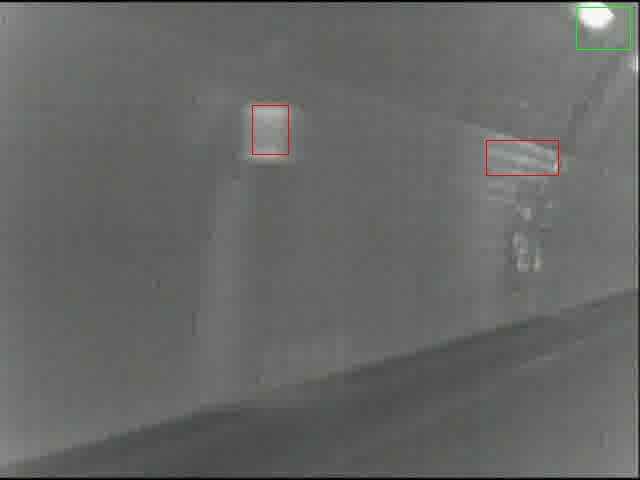
\includegraphics[width=0.47\textwidth,bb=0 0 640 480]{17Rgsimg00039.jpg}
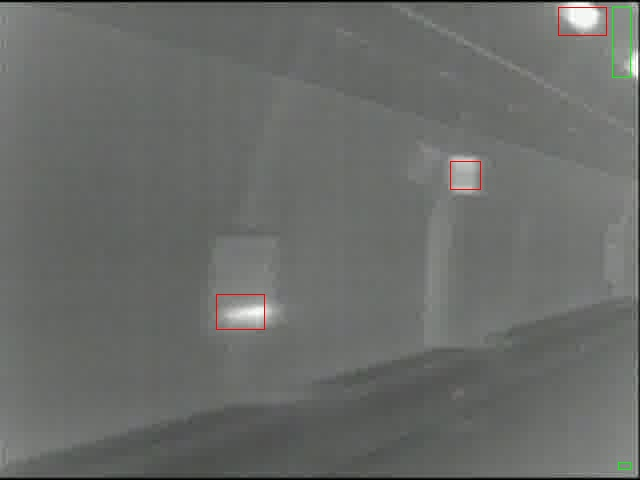
\includegraphics[width=0.47\textwidth,bb=0 0 640 480]{8Rgsimg00028.jpg}
\caption[Keypoint cluster verification by appearance]{Keypoint cluster verification by appearance. Red rectangles: positive detection hypotheses, and green: negative detection hypotheses.}
\label{fig:fiff}
\end{figure}

%test2
\subsection{Keypoint Cluster Tracking}

Not all noisy detection hypotheses can be excluded by using appearance, as shown in Figure \ref{fig:fiff}. To distinguish keypoint clusters belonging to other vehicles and their shadows, the keypoint clusters are tracked through frames to generate trajectories.

In this case of keypoint cluster tracking, the problem is relatively simple, since no occlusion occurs. To keep the method on-line and maintain efficiency, a pool of trajectories are kept, $\tau=\{T_{\bf{g}}^i,i=1,2,...,n\}$, and new detection hypotheses act as detection responses, $\nu=\{n_{\bf{g}}^i,i=1,2,...m\}$, in tracking. The problem of tracking is modeled by finding the best data association hypothesis, $H^*$, between the trajectory set and detection response set as,
\begin{equation}
\begin{aligned}
{H^*} &= \mathop {\arg \max }\limits_{H \in \eta
} (P(H|\tau,\nu )) \\
&= \mathop {\arg \max }\limits_{H \in \eta }
(\prod\limits_{(T_{\bf{g}}^i,n_{\bf{g}}^j) \in H} {P_{link}(n_{\bf{g}}^j|T_{\bf{g}}^i)} ) \;.
\end{aligned}
\label{eq3}
\end{equation}

Let $u_{ij}=1 \mbox{ or } 0$ indicate if $n_{\bf{g}}^j$ is linked to $T_{\bf{g}}^i$ or not, and assuming each trajectory can link once, and each detection response can only be linked once, the problem can be modeled as,
\[
\begin{aligned}
&\arg \max\limits_{u_{ij}} \sum\limits_{i = 1}^n \sum\limits_{j = 1}^m u_{ij} \ln P_{link}(n_{\bf{g}}^j|T_{\bf{g}}^i)\\
&
\begin{aligned}
    s.t.:\mbox{ }&u_{ij}=0\mbox{ or }u_{ij}=1,\forall\;i,\forall\;j;\\
    &\sum\limits_{i = 1}^n {u_{ij}} \leq 1\;; \sum\limits_{j = 1}^m {u_{ij}}\leq 1\;.
\end{aligned}
\end{aligned}
\]
Here, $P_{link}(n_{\bf{g}}^j|T_{\bf{g}}^i)$ is defined by the appearance difference, the scale difference, and the time gap between the last detection response contained in $T_{\bf{g}}^i$ and $n_{\bf{g}}^j$. While the Hungarian algorithm~\citep{ha} gives a near-optimal solution, we follow a very simple manner for the solution by finding the best matched pairs and excluding them until no matching pairs can be found.

\subsection{Keypoint Cluster Verification by Motion}

As shown in Figure \ref{fig:sixs}, the trajectories from keypoint clusters belonging to emergency telephone indicators are different from other objects' trajectories. In this step, the temporal information encoded in the trajectories is used to further verify the keypoint clusters. A linear model is used to fit each trajectory, and the Pearson Correlation Coefficient(PCC) of the fitting is the criteria for the decision.

Let $(x^i_{\bf{g}},y^i_{\bf{g}})$ denote the coordinate of the $i$th element belonging to a trajectory. The linear assumption is that $y^i_{\bf{g}}=a_0+a_1{x^i_{\bf{g}}}$. The PCC of the fitting is defined as,

\begin{equation}
r =| \frac{{\sum\limits_i {\left( {{x^i_{\bf{g}}} -  {\bar x_{\bf{g}}}} \right)\left( {{y^i_{\bf{g}}} -  {\bar y_{\bf{g}}}} \right)} }}{{{{\left[ {\sum\limits_i {{{\left( {{x^i_{\bf{g}}} -  {\bar x_{\bf{g}}}} \right)}^2} \cdot \sum\limits_i {{{\left( {{y^i_{\bf{g}}} -  {\bar y_{\bf{g}}}} \right)}^2}} } } \right]}^{1/2}}}}|\;.
\label{eq4}
\end{equation}
Where $r$ is used to decide if the trajectories of the keypoint clusters belong to emergency telephone indicators or not.
\subsection{Pipeline Summary}
\begin{table}[h]
\centering
\begin{tabular}{lcccc}
     \hline
     \hline
                               & \begin{tabular}{@{}c@{}}Appearance \\ /Motion\end{tabular} & \begin{tabular}{@{}c@{}}Online \\ /Offline\end{tabular} & \begin{tabular}{@{}c@{}}Discriminative \\ /Generative\end{tabular}  \\
    \hline
    Keypoint Detection         &	Appearance & Offline &  Generative  \\
    Keypoint Verification      & Appearance	 & Offline	& Generative \\
    Keypoint Clustering       &	 Appearance  & Online &  \\
    KC Verification by Appearance         &  Appearance    & Offline &  Discriminative	  \\
    KC Tracking                         & Motion & Online &           \\
    KC Verification by Motion           &  Motion    & Online &  Discriminative	   \\
   \hline
\end{tabular}
\caption[Pipeline summary]{Summary of all steps in the pipeline. Here, KC is short for keypoint cluster.}\label{c3tb:tb1}
\end{table}
Before proposing the decision step for detection, Table \ref{c3tb:tb1} summaries the steps in the pipeline based on whether the step employs appearance or motion information, whether the step uses online or offline information, and whether the method is discriminative or generative. Generally speaking, methods that employ motion information and discriminative methods are employed at later steps. This is because the computational cost is high for motion information, and discriminative methods need more information to guarantee performance. Online information are also mainly used in later steps, this is because without information provided by model trained offline, there are no instances to generate online information. Also the computational cost of online information is higher on the fly.


\subsection{Object Detection}

For each keypoint cluster on the current frame, there exists a label given by the Adaboost machine according to its appearance, and the likelihood of fitting its trajectory to a straight line.  For each keypoint cluster, it is considered an emergency telephone indicator if and only if its label - given by the Adaboost machine - is positive, its trajectory is longer than $l^{th}$, and the likelihood of fitting its trajectory to a straight line is larger than $r^{th}$.


\subsection{Voting along a Trajectory}

Each trajectory not only connects the detection responses, but also connects the decisions for detection responses made by their appearance and motion patterns. The target objects and noisy objects actually appear in successive frames, and even if we make a wrong decision on one frame, we can expect to recover from this mistake based on the results of other frames. The final results are based on the trajectories of decisions. When one trajectory ends, if more than 80\% of the decisions it connects are positive, then this trajectory is considered positive.


The procedure is as follows: 1) each detection result along a trajectory which encodes local appearance and motion patterns votes for whether the trajectory is positive or not, and 2) if the voting percentage is larger than a threshold, a final decision is made that the object is positive.



\section{Experimental Results}
\label{exp}
In this section, this method is tested based on detection performance and efficiency. Two experiments  and their results are reported in this section.

\subsection{Experiment One}

\subsubsection{Data} To collect data, infrared cameras are mounted on top of the experimental vehicle, and then we take several tours of the Awagatake tunnel. In the first experiment,  Approximately 4,000 frames are collected for each tour. The frame size is $640\times 480$, the intensity range is [0,255], and the frame rate is 30 frames per second of the camera, and 15 frames per second of the collection program.

\subsubsection{Implementation Settings} All models are trained using data from one tour, while evaluated on data from another tour. Firstly, all emergency telephone indicators are marked in the form of rectangles on all frames from the training tour.

\begin{figure}
\centering
\subfigure[]{
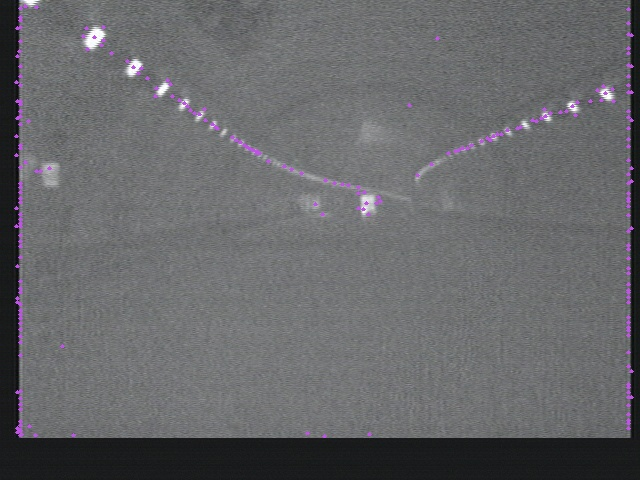
\includegraphics[width=0.47\textwidth,bb=0 0 640 480]{siftimg00469.jpg}
\label{fig:sec:a}}
\subfigure[]{
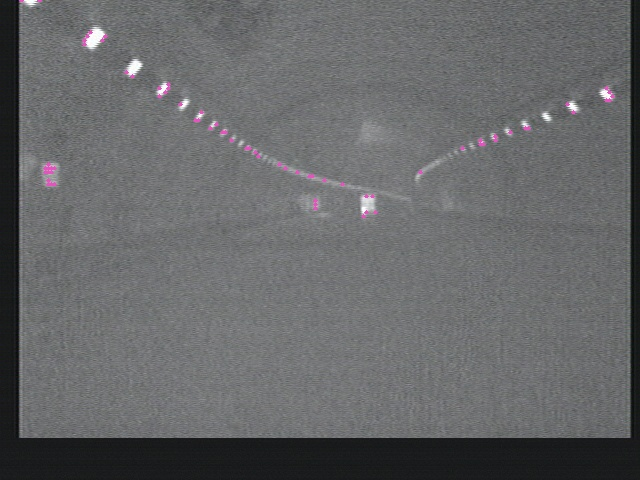
\includegraphics[width=0.47\textwidth,bb=0 0 640 480]{Kptimg00469.jpg}
\label{fig:sec:b}}
\caption[Keypoint detection comparison]{Keypoint detection. In (a), keypoint detection method in~\citep{o12} is used, and in (b), the keypoints are detected using the proposed method. And the proposed keypoint detection is more suitable for detecting keypoints belonging to emergency telephone indicators.}
\label{ex1:va}
\end{figure}


To set intensity thresholds for keypoint detection, a Gaussian distribution is assumed for the intensities of points belonging to target objects. Following the $3\sigma$ principle, $I^{th1}_{\bf{x}}$ is set to 160 and $I^{th2}_{\bf{x}}$ to 190. Width step $W$ set to 3, and $H$ set to 4. Keypoints in the marked rectangle are sampled from the frames of the training tour, are used to estimate $I^{th1}_{\bf{x}}$  and $I^{th2}_{\bf{x}}$.   In Figure \ref{ex1:va}, we also compare the keypoint detection results with the results using SIFT.


  The approximate sub-images of the emergency telephone indicators are manually marked, and used for training the mixture model of keypoint verification. The detected keypoints falling into the sub-image are marked as positive, all other points are marked negative. Note that this model and the training method may not be very accurate, since more accurate marking requires more manual effort.

  Also, future steps can filter out the false alarms produced by this step.  About 30,000 intensity histograms of the positive keypoints are sampled, and about 3,000,000 of the negative. When using of $k$-means for clustering the positive intensity histograms, $k$ is set to 40, and $k$ set to 400 for negative. By using these $k$ values,  both feature sets are over-segmented. The threshold to verify keypoints $D^{th}_{A_{\bf{x}}}$ is set to 0.14 for the normalized histograms.




For keypoint clustering, the threshold to split the mst is set to 10, which is half the largest height of the emergency lights sensed by the camera.

\begin{figure}
\includegraphics[width=1\textwidth,bb=0 0 1367 651]{untitled.jpg}
\caption[Positive and negative training examples]{Dimension reduction of intensity histograms manually marked as positive and negative, which have 2 dimensions by principle component analysis. Blue circles: positive, and red: negative.}
\label{ex1:v}
\end{figure}




 The Adaboost machine to distinguish other vehicles and their shadows is trained by intensity histograms of positive keypoint clusters and negative keypoint clusters. We manually mark 466 positive  and 1,421 negative keypoint clusters. And in Figure \ref{ex1:v}, show the image features of positive and negative training examples for the Adaboost machine, which are reduced to two dimensional by PCA. The trained Adaboost machine is tested on the training dataset, and the classification rate is 85\%.

During keypoint cluster tracking, whether a detection response can be linked to a trajectory or not is constrained by position and scale changes. Here scale change limit is set to 4. When the trajectories are fitted as lines, the linear model is also used in associating new detection responses.


In this experiment, $l^{th}$ is set to 5, $r^{th}$ is set to 0.7, and $R^{th}$ is set to 70\%. As the figures in the section for pipeline are all from the second experiment, here the results of each step of the data from the first experiment are also given. In Figure \ref{ex1:first}, the original data and sample detection results are given. In Figure \ref{ex1:thir}, the results from keypoint verification and clustering are given. In Figure \ref{ex1:four}, the results from keypoint cluster verification by appearance information are given. In Figure \ref{ex1:five}, the results from keypoint cluster tracking are given. And at last, in Figure \ref{ex1:sixs}, the final detection results are given.

\begin{figure}
\centering
\subfigure[]{
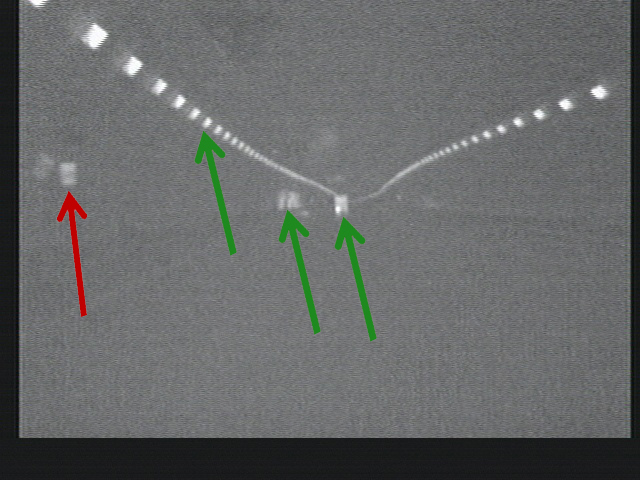
\includegraphics[width=0.47\textwidth,bb=0 0 640 480]{Orgimg00634.jpg}
\label{ex1:first:a}}
\subfigure[]{
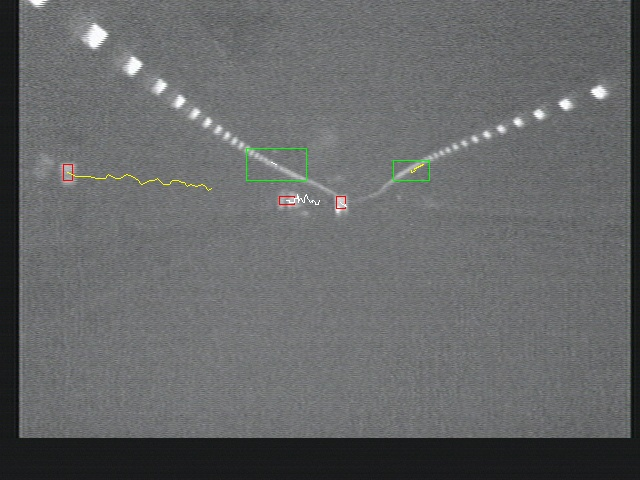
\includegraphics[width=0.47\textwidth,bb=0 0 640 480]{veriRegTrjimg00634.jpg}
\label{ex1:first:b}}
\caption[Original data and detection results]{Original data and detection results. Red arrow points to the target object in \ref{ex1:first:a}.}
\label{ex1:first}
\end{figure}

\begin{figure}
\centering
\subfigure[]{
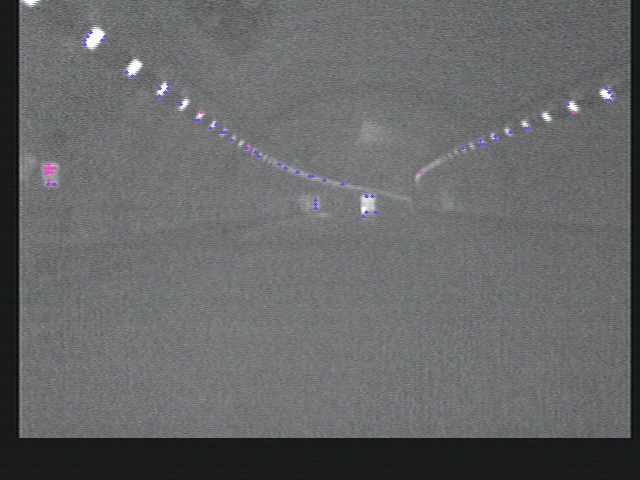
\includegraphics[width=0.47\textwidth,bb=0 0 640 480]{VeriKptimg00469.jpg}
\label{fig:thir:a}}
\subfigure[]{
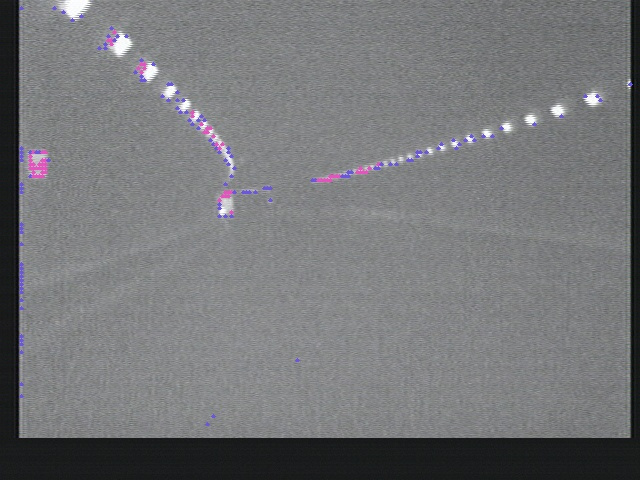
\includegraphics[width=0.47\textwidth,bb=0 0 640 480]{VeriKptimg01080.jpg}
\label{fig:thir:b}}
\subfigure[]{
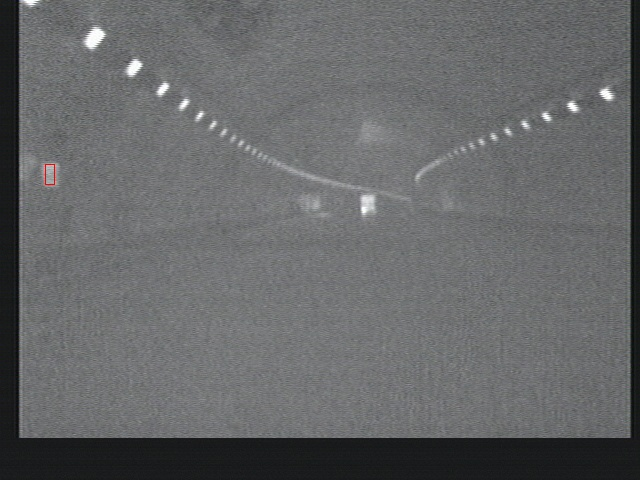
\includegraphics[width=0.47\textwidth,bb=0 0 640 480]{Rgsimg00469.jpg}
\label{fig:thir:c}}
\subfigure[]{
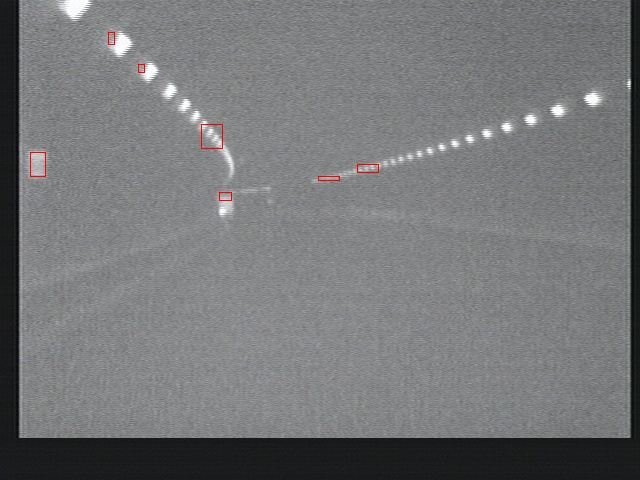
\includegraphics[width=0.47\textwidth,bb=0 0 640 480]{Rgsimg01080.jpg}
\label{fig:thir:d}}
\caption[Keypoint verification and clustering]{Keypoint verification and clustering. }
\label{ex1:thir}
\end{figure}

\begin{figure}[b]
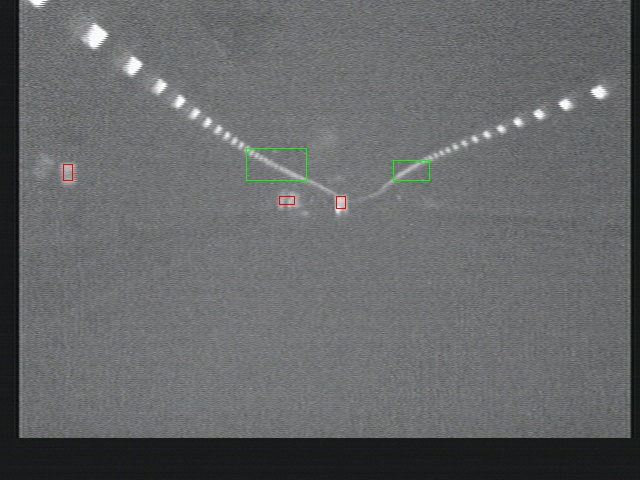
\includegraphics[width=0.47\textwidth,bb=0 0 640 480]{VeriRgsimg00634.jpg}
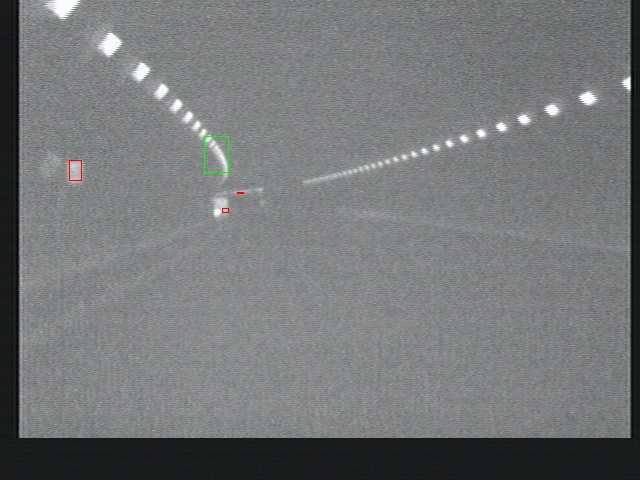
\includegraphics[width=0.47\textwidth,bb=0 0 640 480]{VeriRgsimg01075.jpg}
\caption[Keypoint cluster verification by appearance]{Keypoint cluster verification by appearance. Red rectangles: positive detection hypotheses, and green: negative detection hypotheses.}
\label{ex1:four}
\end{figure}

\begin{figure}
{
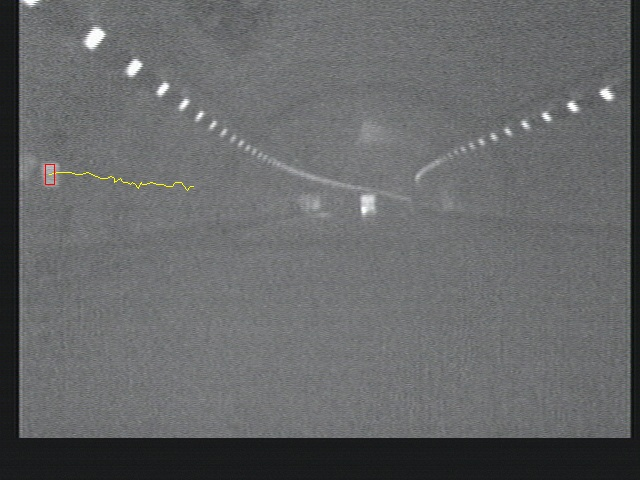
\includegraphics[width=0.47\textwidth,bb=0 0 640 480]{Trjimg00469.jpg}
}
{
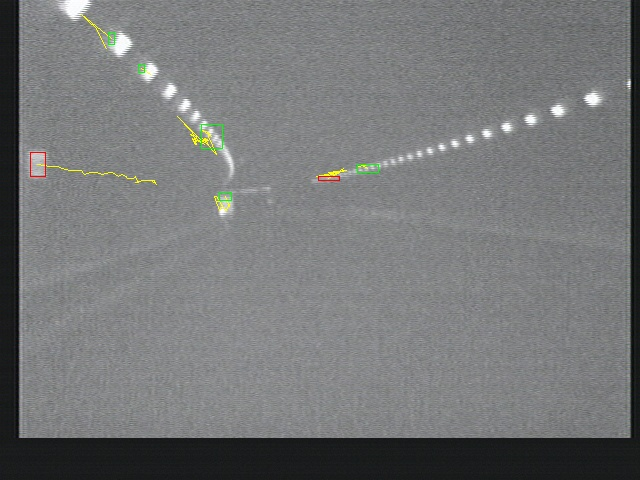
\includegraphics[width=0.47\textwidth,bb=0 0 640 480]{Trjimg01080.jpg}
}
\caption[Keypoint cluster tracking]{Keypoint cluster tracking.}
\label{ex1:five}
\end{figure}

\begin{figure}
{
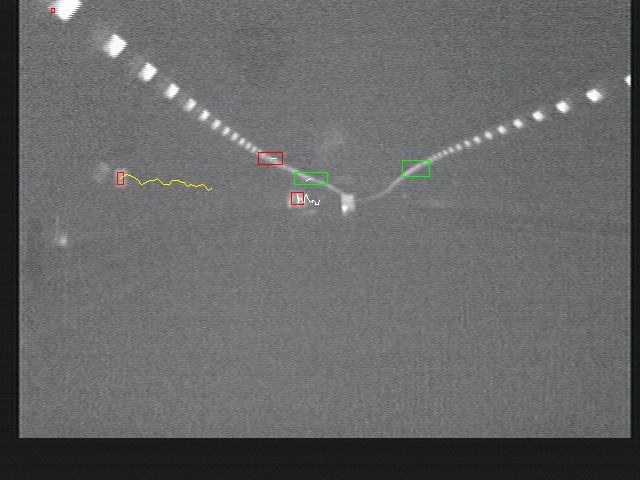
\includegraphics[width=0.47\textwidth,bb=0 0 640 480]{veriRegTrjimg00626.jpg}
}
{
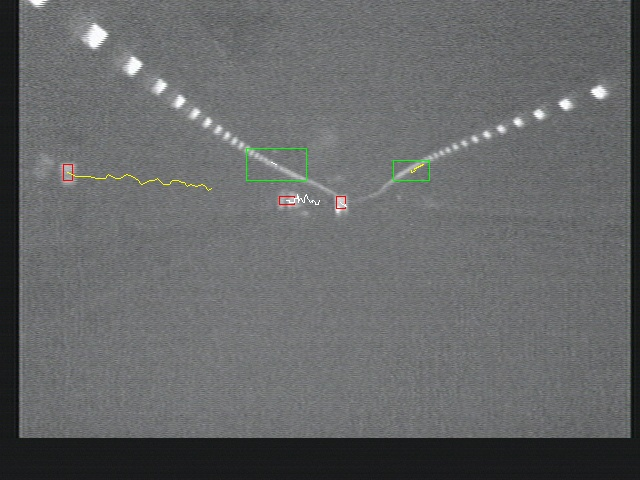
\includegraphics[width=0.47\textwidth,bb=0 0 640 480]{veriRegTrjimg00634.jpg}
}\\
{
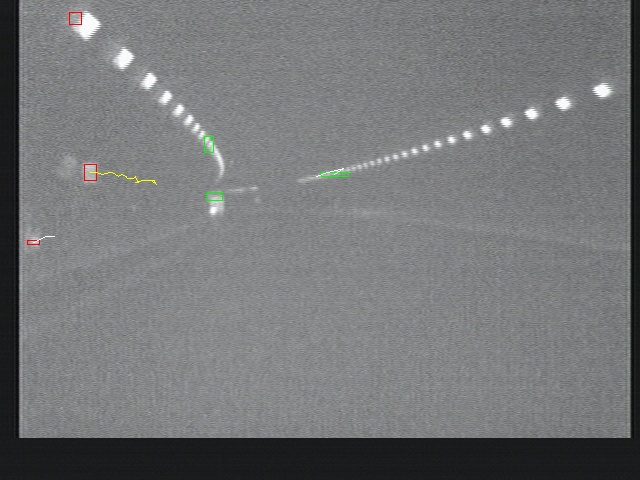
\includegraphics[width=0.47\textwidth,bb=0 0 640 480]{veriRegTrjimg01072.jpg}
}
{
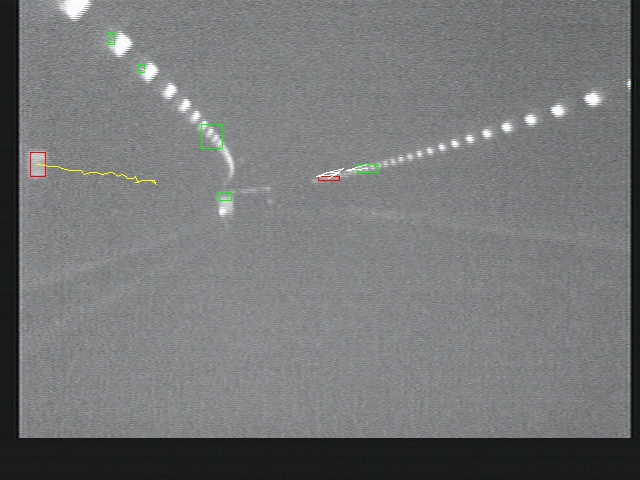
\includegraphics[width=0.47\textwidth,bb=0 0 640 480]{veriRegTrjimg01080.jpg}
}
\caption[Detection results]{Detection results.}
\label{ex1:sixs}
\end{figure}

\subsubsection{Detection Results} On a laptop with Intel Core2 Duo 2.8GHz processors, the method deals with real data at a frame rate of 34 frames per second, and this fulfills real-time requirements.

The detection rate and false alarm rate is evaluated on 250 frames, as shown in Table \ref{ex1:tb2}.

\begin{table}[h]
\centering
\begin{tabular}{lll}
     \hline
     \hline
    Total number &	113   \\
    Correctly labeled &	102   \\
    Miss detections &	11 &	  \\
    False alarms &	21    \\
    Detection rate &	90\% &	  \\
    False alarm rate &	19\% &	   \\
   \hline
\end{tabular}
\caption[Detection rate and false alarm rate]{Detection rate and false alarm rate.}\label{ex1:tb2}
\end{table}

\subsection{Experiment Two}



\subsubsection{Data} The results of the first experiment is not satisfactory, and then the second experiment is carried out. A better far infrared camera is used, and the zoom of the camera is adjusted for better images. Then with the new camera mounted on top, the experimental vehicle took several tours of the Awagatake tunnel. About 7,000 frames are collected for each tour. The frame size is $640\times 480$, the intensity range is [0,255], and the frame rate is 30 frames per second of the camera, also of the data collection program which is provided by the camera maker.

\subsubsection{Implementation Settings} Being the same with experiment one, all models are trained using data from one tour, and evaluated on data on another tour.

 For keypoint detection, $I^{th1}_{\bf{x}}$ is set to 160 and $I^{th2}_{\bf{x}}$, 190. According to the sensed emergency telephone indicator, width step $W$ set to 3, and $H$ set to 4.

Instead of training a new mixture model for keypoint verification, the older one from experiment one is used, since the performance of this step is not critical.

For keypoint clustering, the threshold to split the mst is set to 40, which is half the largest height of the emergency telephone indicators sensed with new camera and experimental settings.


The Adaboost machine used to distinguish other vehicles and their shadows is trained by intensity histograms of positive keypoint clusters and negative keypoint clusters. We manually mark  positive  and  negative keypoint clusters. If the Adaboost machine is trained by averagely weighted training examples, its correct rate on the training examples is overall 84\%. When trained using this bias weighted training examples, its correct rate is  94\% for the positive training examples, and 77\% for the negative training examples.
During keypoint cluster tracking, whether a detection response can be linked to a trajectory or not is constrained by position and scale changes. Here scale change limit is set to 4. When the trajectories are fitted as lines, the linear model is also used in associating new detection responses.

The main difference with experiment one in the pipeline here is how the Adaboost machine is trained. The same weights are assigned to positive and negative training examples during training the Adaboost machine in experiment one, while biased weights are assigned here. This will results in an Adaboost machine which gives better performance on target objects, and perform worse on noisy objects. The produced false alarms can be  filtered out by a more powerful later step which uses motion information.

During keypoint cluster tracking, whether a detection response can be linked to a trajectory or not is constrained by position and scale changes. Here scale change limit is set to 4. When the trajectories are fitted as lines, the linear model is also used in associating new detection responses.



\begin{figure}
{
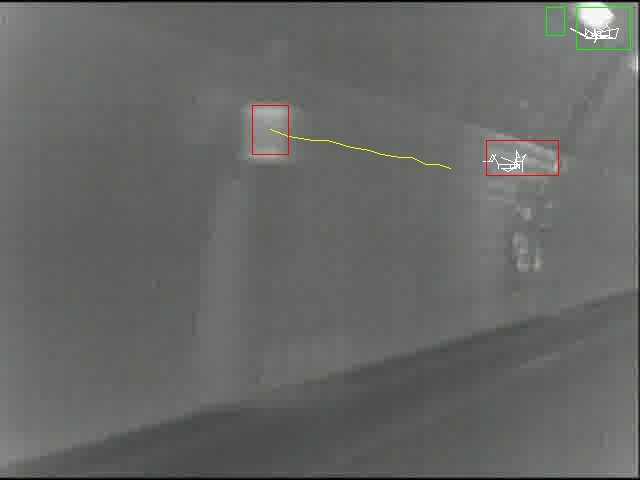
\includegraphics[width=0.47\textwidth,bb=0 0 640 480]{17veriTrjimg00039.jpg}
}
{
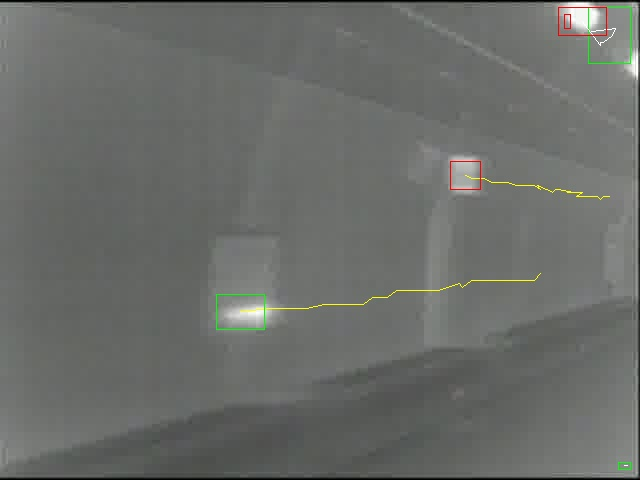
\includegraphics[width=0.47\textwidth,bb=0 0 640 480]{8veriTrjimg00028.jpg}
}\\
{
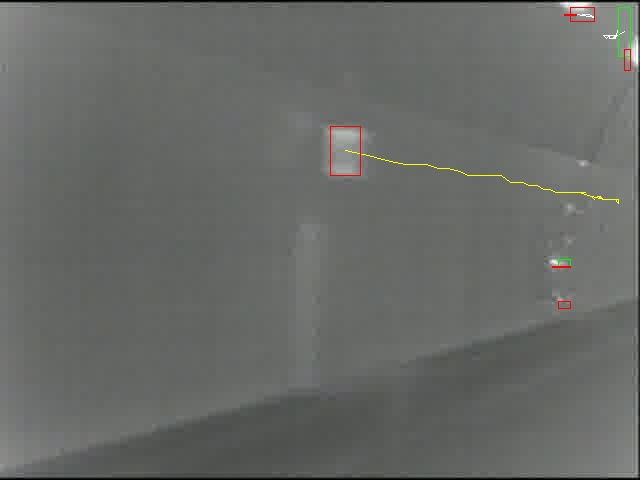
\includegraphics[width=0.47\textwidth,bb=0 0 640 480]{19veriTrjimg00041.jpg}
}
{
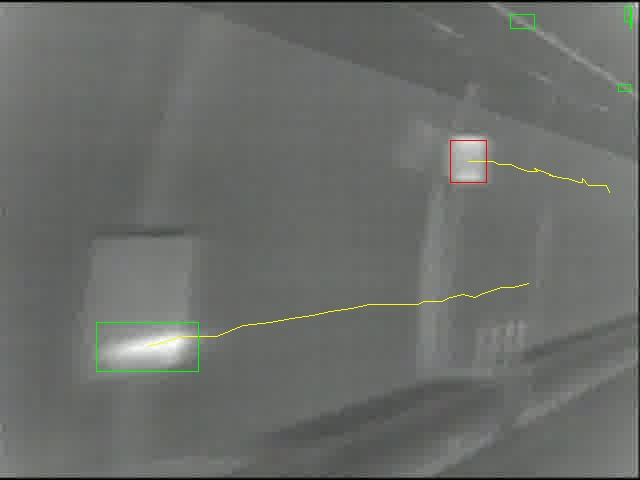
\includegraphics[width=0.47\textwidth,bb=0 0 640 480]{3veriTrjimg00023.jpg}
}\\
{
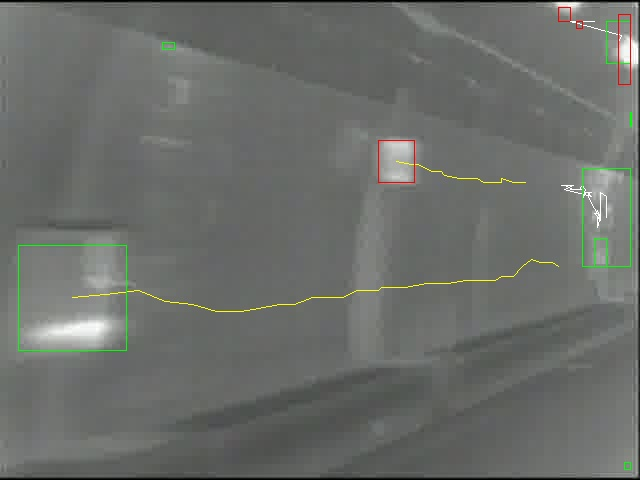
\includegraphics[width=0.47\textwidth,bb=0 0 640 480]{04veriTrjimg00039.jpg}
}
{
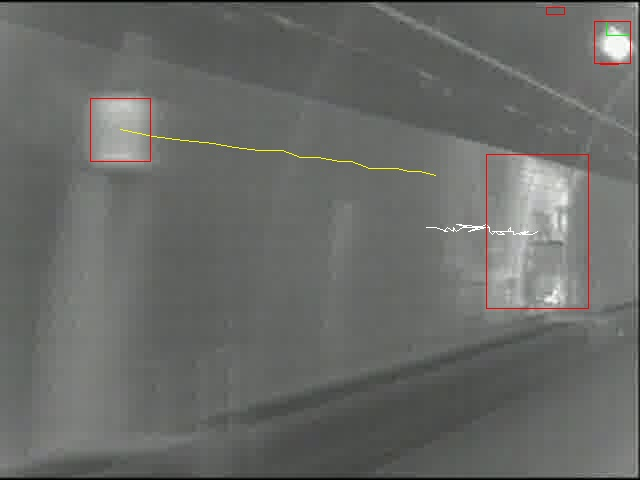
\includegraphics[width=0.47\textwidth,bb=0 0 640 480]{02veriTrjimg00046.jpg}
}\\
{
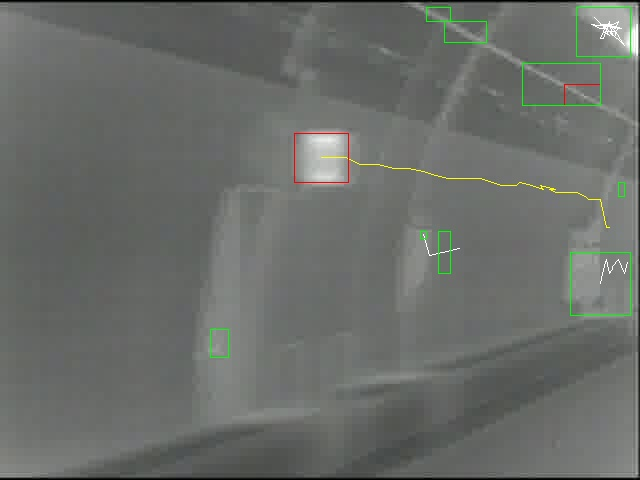
\includegraphics[width=0.47\textwidth,bb=0 0 640 480]{00veriTrjimg00032.jpg}
}
{
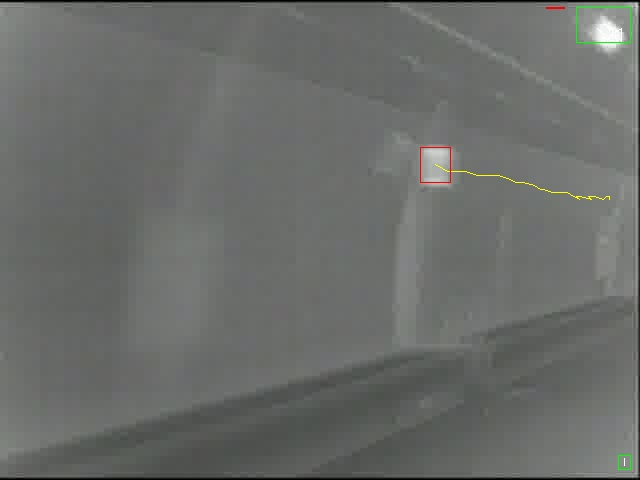
\includegraphics[width=0.47\textwidth,bb=0 0 640 480]{06veriTrjimg00032.jpg}
}

\caption[Detection results]{Detection results.}
\label{fig:sixs}
\end{figure}

\subsubsection{Detection Results}

Using an ordinary desktop computer with Intel Core2 Quad 2.6GHz processors, the method deals with real data at a frame rate of 41 frames per second, and this fulfills real-time requirements.


The detection rate and false alarm rate are evaluated on the keypoint clusters, as shown in Table \ref{tb:tb2}.
More detection results are shown in Figure \ref{fig:sixs}.
\begin{table}[h]
\centering
\begin{tabular}{lll}
     \hline
     \hline
    Total number &	472  \\
    Correctly labeled &	468   \\
    Miss detections &	4 &	  \\
    False alarms &	22    \\
    Detection rate &	99.2\% &	  \\
    False alarm rate &	4.4\% &	   \\
   \hline
\end{tabular}
\caption[Detection rate and false alarm rate]{Detection rate and false alarm rate.}\label{tb:tb2}
\end{table}





The detection rate and false alarm rate of the first experiment~\citep{wang1} are 90\% and 19\%, while evaluated on a much smaller dataset. Here the results are better than   experiment one, because the sensed images are much clearer, and because this more effective training of the Adaboost machine.

The results on the trajectories of decisions are also evaluated. When one trajectory ends, if its length is larger than 15, and over 80\% of the last 15 decisions it connects are positive, it is considered as positive. The method correctly detects all the 22 emergency telephone indicators with no false alarms. The detection rate is 100\%, and the false alarm rate is 0\%, as shown in Table \ref{tb:tb3}.

\begin{table}[h]
\centering
\begin{tabular}{lll}
     \hline
     \hline
   Total number & 22  \\
    Correctly labeled &	22   \\
    Miss detections &	0 &	  \\
    False alarms &	0    \\
    Detection rate &	100\% &	  \\
    False alarm rate &	0\% &	   \\
   \hline
\end{tabular}
\caption[Final detection rate and false alarm rate]{Final detection rate and false alarm rate.}\label{tb:tb3}
\end{table}

\section{Experimental results on data collected by ordinary cameras}
\label{ord}




\begin{figure}
{
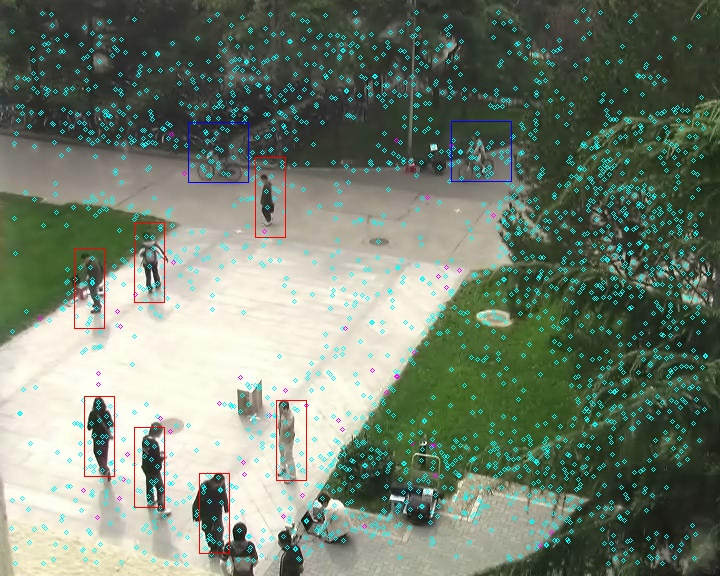
\includegraphics[width=0.47\textwidth,bb=0 0 720 576]{frame92_af.jpg}
}
{
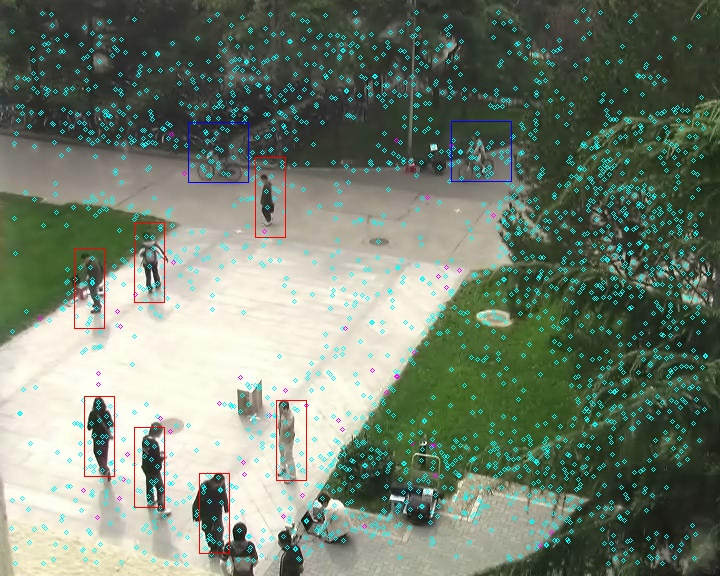
\includegraphics[width=0.47\textwidth,bb=0 0 720 576]{frame92_af.jpg}
}\\

\caption[Keypoint verification]{Results of keypoint verification. Rectangles mark the manually marked ground-truth boxes. Pink points mark the points labeled as negative in keypoint verification step, others mark keypoints of the positive. }
\label{ord:two}
\end{figure}
The method is extended at the first step to deal with data collected by ordinary cameras. The task is to detect pedestrians and bicycle riders. SURF~\citep{surf} is used as keypoint detector and descriptor.

A new keypoint verification step is proposed. Keypoints from training examples are clustered using $k$-means as a mixture model. Gaussian distribution is assumed for each cluster, and the variances are also estimated, which will be used as criteria for keypoint verification. Different $k$s are used to generate the mixture model, and the performance is evaluated in Figure \ref{ord:one}.  An ensemble model is proposed, which never performs worst. All results of $k$-means with different parameters are summarised to produce the results of ensemble model.

As shown in Figure \ref{ord:two}, keypoint detection step is performing good in detect keypoints belonging to the target objects. The performance of keypoint verification is not good, as shown in Figure \ref{ord:one}. And this leads to infeasible later steps.

The failure of this method in complex scene is the lacking of descriptive power in its model. Beside appearance information, the positional information is also important when talking about complex scenes.

\begin{figure}
\centering
{
  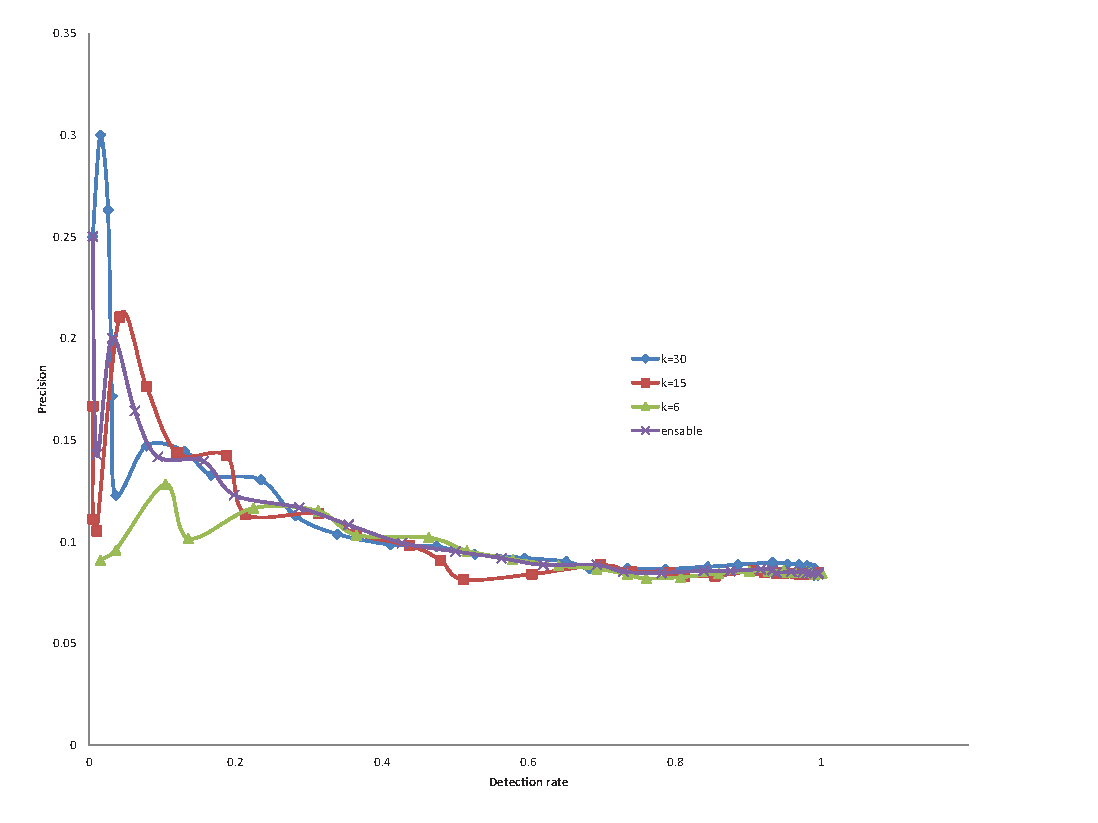
\includegraphics[width=1\textwidth]{kptkms.eps}
}
\caption[Evaluation of keypoint verification]{Evaluation of keypoint verification. Keypoint verification performance of $k$-means mixture models with different parameters. Here, $k$ is the main parameter, while the model of ensemble uses all mixture models.}
\label{ord:one}
\end{figure}

\section{Chapter Conclusion}
\label{conc}
 This chapter proposes an object detection method, which performs well in simple scenarios by combining appearance and motion information in a very efficient way. The method makes use of appearance and motion information of the target objects in a hierarchical manner. With careful optimization of detection pipeline, the method gives promising results in real time.

  Also one main idea of the method is not to consider objects as something only with specific appearance patterns, but as something with both
 specific appearance and motion patterns. Another reason for the performance during the second experiment, is that make dangerous decisions later, when more information are available. While using both appearance and motion information results in a detection rate of about 99\%.

 Though its performance under complex scenarios is not promising, it can still be used as a unit in  positioning systems in tunnel environment.
